\documentclass[11pt]{article}
\usepackage[utf8]{inputenc}
\usepackage{amsmath,amssymb}
\usepackage{graphicx}
\usepackage{booktabs}
\usepackage{authblk}
\usepackage[margin=1in]{geometry}
\usepackage[hidelinks]{hyperref}
\usepackage{xurl}
\usepackage{setspace}
\usepackage{tikz}
\usetikzlibrary{arrows.meta,positioning}

\title{A Coulomb Route to Solar Fusion:\\
$p+e+p\to d$ and $d+d\to{}^4$He}
\author[1]{Claes Johnson}
\affil[1]{KTH Royal Institute of Technology, SE-100 44 Stockholm, Sweden \\
\texttt{claesjohnson@gmail.com}}
\date{\today \\[0.4em]
\small\textit{Physical argument by the author; numerical implementation with AI assistance (Claude, Anthropic).}}

\begin{document}
\maketitle

\begin{abstract}
In the standard proton--proton chain, solar hydrogen burning begins with $p+p\to d+e^{+}+\nu_e$, a
\emph{weak}-force reaction that converts a proton into a neutron with emission of a positron and a
neutrino, and is the slow, rate-limiting step of the whole chain. In the RealNucleus picture --- in
which the neutron is a bound proton--electron pair and the deuteron is $2p+1e$ --- the same first step
is purely \emph{electromagnetic}: $p+e+p\to d$, an electron from the plasma captured as the deuteron's
glue, with no flavour change, no positron, and no neutrino. Two deuterons then fuse to the alpha,
$d+d\to{}^4$He, a reaction computed directly in RealQM. The net process $4p+2e\to{}^4\mathrm{He}$
releases the same ${\sim}26.7$~MeV as the standard chain but retains the ${\sim}0.5$~MeV per alpha
(${\sim}2\%$) that the standard chain loses to neutrinos. The decisive difference is a lepton one: in
RealNucleus no lepton is created or destroyed --- the electron persists as the deuteron's constituent
--- so lepton-number conservation requires \emph{no} neutrino, whereas the standard neutrino is the
signature of the flavour-changing weak vertex $p\to n$. We set the two schemes side by side and
identify the experimentum crucis: the solar neutrino flux, directly measured, which the standard weak
picture predicts and which the Coulomb picture must account for. The comparison is thus sharp and
falsifiable.

\medskip
\noindent\textbf{Keywords:} solar fusion; proton--proton chain; deuteron formation; electron capture;
RealNucleus; weak force; solar neutrinos; hydrogen burning.
\end{abstract}

\setstretch{1.12}

\section{Introduction}

The Sun shines by fusing hydrogen to helium, $4p\to{}^4\mathrm{He}$, releasing $26.73$~MeV per helium
nucleus. In the standard account~\cite{Bethe,Adelberger} this proceeds through the
proton--proton (pp) chain, whose first and rate-limiting step,
\begin{equation}
p + p \;\longrightarrow\; d + e^{+} + \nu_e ,
\label{eq:pp}
\end{equation}
is a \emph{weak}-interaction process: two protons collide, one is converted to a neutron
($p\to n + e^{+} + \nu_e$), and the resulting proton and neutron bind as a deuteron. Because it
requires the weak force acting during the brief instant two protons are within nuclear range, this
step is extraordinarily slow --- it is what makes the Sun's hydrogen last billions of years --- and it
emits a neutrino that escapes the Sun directly.

RealNucleus~\cite{Johnson-RealNucleus,Johnson-RealQM} offers a different account of the same burning.
There the neutron is not elementary but a bound proton--electron pair, $n=(p\,e^-)$, and the deuteron
is accordingly $2p+1e$: two protons glued by a single shared electron, the charge-conjugate of the
one-electron molecular ion $\mathrm{H}_2^{+}$. In this picture the first step of hydrogen burning is
not weak but electromagnetic,
\begin{equation}
p + e + p \;\longrightarrow\; d ,
\label{eq:pep}
\end{equation}
an electron drawn from the surrounding plasma and captured as the deuteron's glue --- no proton is
converted, no positron is created, and no neutrino is required. The chain then closes with the direct
fusion of two deuterons,
\begin{equation}
d + d \;\longrightarrow\; {}^4\mathrm{He} ,
\label{eq:dd}
\end{equation}
a reaction we have computed directly in RealQM~\cite{Johnson-RealNucleus}. This paper places the two
accounts side by side, compares their energetics and their lepton content, and identifies the single
measurement that decides between them.

\section{The standard proton--proton chain}

The dominant (ppI) branch of the standard chain is
\begin{align}
p + p &\to d + e^{+} + \nu_e && (Q = 0.42~\text{MeV};\ \text{weak, rate-limiting}),\\
d + p &\to {}^3\mathrm{He} + \gamma && (Q = 5.49~\text{MeV}),\\
{}^3\mathrm{He} + {}^3\mathrm{He} &\to {}^4\mathrm{He} + 2p && (Q = 12.86~\text{MeV}),
\end{align}
with the two positrons annihilating on plasma electrons. Summing the branch and the annihilations, the
net is
\begin{equation}
4p + 2e^- \;\longrightarrow\; {}^4\mathrm{He} + 2\nu_e + 26.73~\text{MeV},
\label{eq:standard-net}
\end{equation}
of which the two neutrinos carry away, on average, ${\sim}0.5$~MeV, so that ${\sim}26.2$~MeV is
deposited as heat. The rate is set by two factors in series: the Coulomb barrier the two protons must
tunnel (the Gamow factor, steeply temperature-dependent), \emph{and} the weak matrix element for
$p\to n$ conversion during the collision. The second factor is tiny, and it is the weak bottleneck ---
not the Coulomb barrier alone --- that fixes the Sun's luminosity and lifetime. A minor variant, the
\emph{pep} reaction $p+e^-+p\to d+\nu_e$ (about $0.4\%$ of pp), captures a plasma electron instead of
emitting a positron, but is still weak and still emits a neutrino.

\begin{figure}[t]
\centering
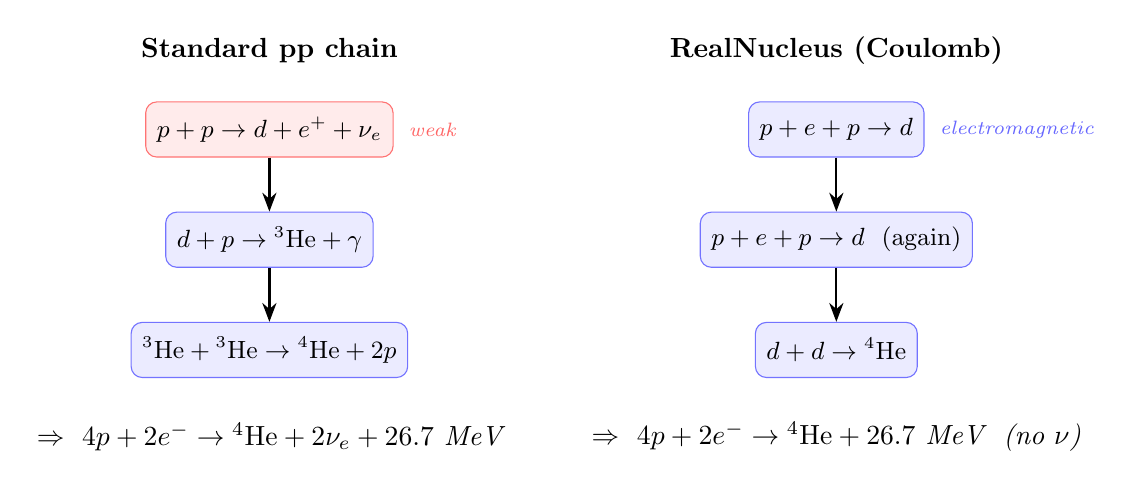
\begin{tikzpicture}[
  font=\small,
  box/.style={draw,rounded corners,inner sep=4pt,minimum height=7mm,align=center},
  wk/.style={box,fill=red!8,draw=red!55},
  em/.style={box,fill=blue!8,draw=blue!55},
  ar/.style={-{Stealth[length=2.4mm]},thick},
  lab/.style={font=\scriptsize\itshape}]

 % ---- standard column ----
 \node[align=center,font=\bfseries] at (0,1.0) {Standard pp chain};
 \node[wk] (s1) at (0,0) {$p+p\to d+e^{+}+\nu_e$};
 \node[lab,red!60,right=2pt of s1] {weak};
 \node[em] (s2) at (0,-1.4) {$d+p\to{}^3\mathrm{He}+\gamma$};
 \node[em] (s3) at (0,-2.8) {${}^3\mathrm{He}+{}^3\mathrm{He}\to{}^4\mathrm{He}+2p$};
 \draw[ar] (s1) -- (s2);
 \draw[ar] (s2) -- (s3);
 \node[align=center,font=\itshape] at (0,-3.9) {$\Rightarrow\ 4p+2e^-\to{}^4\mathrm{He}+2\nu_e+26.7$~MeV};

 % ---- RealNucleus column ----
 \node[align=center,font=\bfseries] at (7.2,1.0) {RealNucleus (Coulomb)};
 \node[em] (r1) at (7.2,0) {$p+e+p\to d$};
 \node[lab,blue!60,right=2pt of r1] {electromagnetic};
 \node[em] (r2) at (7.2,-1.4) {$p+e+p\to d$\ \ (again)};
 \node[em] (r3) at (7.2,-2.8) {$d+d\to{}^4\mathrm{He}$};
 \draw[ar] (r1) -- (r2);
 \draw[ar] (r2) -- (r3);
 \node[align=center,font=\itshape] at (7.2,-3.9) {$\Rightarrow\ 4p+2e^-\to{}^4\mathrm{He}+26.7$~MeV\ \ (no $\nu$)};
\end{tikzpicture}
\caption{The two accounts of solar hydrogen burning. \emph{Left:} the standard pp chain opens with the
weak reaction $p+p\to d+e^{+}+\nu_e$ (red), which converts a proton to a neutron and emits a neutrino.
\emph{Right:} the RealNucleus chain opens with the electromagnetic capture $p+e+p\to d$ (blue), the
electron becoming the deuteron's glue, and closes with the directly-computed $d+d\to{}^4$He. Both net
to $4p+2e^-\to{}^4$He at $26.7$~MeV; only the standard chain emits neutrinos.}
\label{fig:chains}
\end{figure}

\section{The Coulomb route}

In RealNucleus the ground state of a nucleus is a set of proton and electron charge clouds on
non-overlapping domains with free boundaries, minimising the Coulomb (electrostatic) energy alone,
\begin{equation}
E \;=\; \sum_i \tfrac{1}{2}\!\int|\nabla\psi_i|^2
\;+\; \tfrac12\!\iint\frac{\rho(x)\rho(y)}{|x-y|}\,dx\,dy, \qquad \rho=\sum_i q_i\psi_i^2 ,
\label{eq:energy}
\end{equation}
with $q_i=\pm1$~\cite{Johnson-RealQM,Johnson-RealNucleus}. A free proton and a free electron form the
model neutron $1p+1e$, which does \emph{not} bind on its own (matching the instability of the free
neutron); but a \emph{second} proton produces the deuteron $2p+1e$, which does. The single electron
cannot glue one proton into a bound unit yet glues two --- the charge-conjugate $\mathrm{H}^-$/
$\mathrm{H}_2^{+}$ configuration, the two protons splitting into halfspaces around the central electron
core. This is the reaction~\eqref{eq:pep}: it needs only an electron, always abundant in the solar
plasma, and the Coulomb attraction that binds it; no proton is transmuted.

The second step~\eqref{eq:dd}, $d+d\to{}^4\mathrm{He}$, is the fusion of two such units into the alpha
$4p+2e$ --- the closed, dual-confined structure in which a $-2$ electron core is caged by four
protons. In RealQM this reaction is computed directly: two deuterons, each a central electron core
with its two protons split into halfspaces, are brought together and relaxed, and the energy falls
monotonically onto the deeply bound alpha as the separation decreases~\cite{Johnson-RealNucleus}. The
overall balance is
\begin{equation}
4p + 2e^- \;\longrightarrow\; {}^4\mathrm{He} + 26.73~\text{MeV},
\label{eq:coulomb-net}
\end{equation}
identical in energy to the standard net~\eqref{eq:standard-net} except that no energy is carried off by
neutrinos.

\paragraph{Which second step?} A caveat on abundances is in order. In the solar core protons outnumber
deuterons enormously: a deuteron, once formed, is consumed almost at once, so its equilibrium
abundance is only $[d]/[p]\sim10^{-18}$. In the standard chain this is precisely why deuterium burns by
$d+p\to{}^3\mathrm{He}$ and not by $d+d$, which is utterly negligible. The same abundance argument
applies to the Coulomb route: the dominant second step in a proton-rich plasma is likewise
$d+p\to{}^3\mathrm{He}$ --- in RealNucleus simply $3p+1e$, again electromagnetic --- followed by
${}^3\mathrm{He}+{}^3\mathrm{He}\to{}^4\mathrm{He}+2p$, exactly the ppI topology but with every step
Coulombic and neutrino-free. We write the chain as $d+d\to{}^4\mathrm{He}$ in~\eqref{eq:dd} because that
reaction is the one computed directly in RealQM~\cite{Johnson-RealNucleus} and the cleanest picture of
two dual-confined units merging into the closed alpha; the abundance-weighted path through
${}^3\mathrm{He}$ tells the same electromagnetic story, $4p+2e^-\to{}^4\mathrm{He}$, and is equally free
of the weak vertex. The essential contrast with the standard chain therefore lies entirely in the
\emph{first} step, the formation of the deuteron: whether it is the weak $p+p\to d+e^{+}+\nu_e$ or the
electromagnetic $p+e+p\to d$. Every step thereafter is Coulombic in both accounts; only the entry point
carries --- or does not carry --- the neutrino.

\section{Comparison}

Table~\ref{tab:compare} sets the two accounts against each other. They agree on the overall
transmutation and on its energy release; they differ on the \emph{mechanism} of the first step, and
hence on the leptons and the neutrinos.

\begin{table}[h]
\centering
\renewcommand{\arraystretch}{1.25}
\begin{tabular}{lll}
\toprule
 & \textbf{Standard pp chain} & \textbf{RealNucleus (Coulomb)}\\
\midrule
first step        & $p+p\to d+e^{+}+\nu_e$      & $p+e+p\to d$\\
force             & weak (flavour-changing $p\to n$) & electromagnetic (Coulomb)\\
what the deuteron is & $p+n$, $n$ elementary     & $2p+1e$, $n=(p\,e^-)$ bound\\
second step       & $d+p\to{}^3$He, then ${}^3$He$+{}^3$He & $d+d\to{}^4$He (computed)\\
leptons           & $e^{+}$ and $\nu_e$ created   & electron retained; none created\\
neutrinos         & yes ($2\,\nu_e$ per $^4$He)  & none\\
net               & $4p+2e^-\to{}^4$He$+2\nu_e$   & $4p+2e^-\to{}^4$He\\
energy            & $26.73$~MeV ($\sim0.5$ to $\nu$) & $26.73$~MeV (all retained)\\
rate limiter      & weak vertex $\times$ Coulomb barrier & Coulomb barrier (three-body $p e p$)\\
\bottomrule
\end{tabular}
\caption{The standard proton--proton chain and the RealNucleus Coulomb route to solar hydrogen
burning, step by step.}
\label{tab:compare}
\end{table}

\paragraph{The lepton argument.} The cleanest distinction is one of lepton bookkeeping. In the standard
first step a proton is turned into a neutron, a flavour-changing weak transition that must create a
positron and a neutrino to conserve charge and lepton number: the neutrino is the \emph{signature of
the weak vertex}. In the Coulomb route no proton is transmuted and no lepton is created or destroyed
--- the plasma electron simply becomes the deuteron's glue and remains as the constituent electron of
the $n=(p\,e^-)$ pair. Lepton number is then conserved trivially, with no neutrino. The presence or
absence of the solar neutrino is thus a direct readout of which mechanism operates.

\section{Energetics and the neutrino budget}

Both routes conserve energy at the same value because both effect the same net transmutation
$4p+2e^-\to{}^4\mathrm{He}$, whose $Q$-value is fixed by the masses,
\begin{equation}
Q = \big(4m_p + 2m_e - m_{^4\mathrm{He}}\big)c^2
  = (3753.09 + 1.02 - 3727.38)~\text{MeV} = 26.73~\text{MeV}.
\end{equation}
The standard chain gives up about $0.5$~MeV of this to its two neutrinos (mean pp-neutrino energy
$\approx 0.27$~MeV each), so $\approx 26.2$~MeV becomes solar heat and light; the Coulomb route retains
the full $26.73$~MeV. Equivalently, the standard model predicts a solar \emph{neutrino luminosity} of
about $2\%$ of the total, while the Coulomb route predicts essentially none. This few-percent split is
small in the energy budget but it is the whole of the observable neutrino signal.

\section{The decisive test: solar neutrinos}
\label{sec:test}

Here the comparison becomes an experiment, and honesty requires stating the current evidence plainly.
The standard chain predicts a pp-neutrino flux at Earth of about
$6\times10^{10}~\mathrm{cm^{-2}\,s^{-1}}$, tied directly to the solar luminosity, and solar neutrinos
are \emph{observed}: the chlorine and gallium radiochemical experiments, Super-Kamiokande and SNO
(which established flavour oscillation and measured the total ${}^8$B flux), and above all Borexino,
which has directly measured the low-energy pp, ${}^7$Be and pep neutrinos in real time at fluxes
consistent with the standard solar model~\cite{Borexino,SNO,Adelberger}. Detection is by
neutrino--electron scattering and inverse beta decay, which count arriving neutrinos in a largely
production-model-independent way. Taken at face value, this flux is strong evidence for a
neutrino-emitting --- hence weak --- first step, and it is the principal challenge the Coulomb route
must meet: a strictly neutrino-free burning is disfavoured by the measured flux unless that flux can be
attributed to another source.

We therefore state the position without overreach. The Coulomb route is a well-defined, computable, and
energetically exact account of $4p+2e^-\to{}^4\mathrm{He}$ that removes the awkward features of the
weak first step --- the unbound diproton, the improbable in-flight $p\to n$ conversion --- and predicts
a specific, falsifiable consequence: little or no solar neutrino emission from the initial deuteron
formation. The measured pp-neutrino flux is the experimentum crucis. If that flux is genuinely of
primary solar origin at the standard-model value, the strictly neutrino-free version is excluded and
any Coulomb account must incorporate a neutrino-producing channel; if some part of the inferred flux
rests on assumptions about the production mechanism, that part is open to reexamination. Either way the
question is settled by measurement, not by preference --- which is the proper standing of a physical
proposal.

\section{The original need for the neutrino, and whether it disappears}

Pauli's neutrino of 1930 was a \emph{desperate remedy}~\cite{Pauli}: a particle postulated solely to
rescue two conservation laws that beta decay appeared to violate. First, \emph{energy and momentum} ---
the beta electron emerges with a \emph{continuous} spectrum, whereas a two-body decay $n\to p+e$ would
make it monoenergetic, so a third, unseen body must carry the balance. Second, \emph{angular momentum
and statistics} --- the neutron is spin-$\tfrac12$, but $n\to p+e$ yields spin $0$ or $1$ (two fermions
make a boson), so a third spin-$\tfrac12$ fermion is needed to restore both the half-integer spin and
the fermionic statistics. Pauli's neutrino supplied both at a stroke, and went undetected for a
generation. Two questions then separate: whether the present picture \emph{needs} the neutrino, and
whether the \emph{original} need is still what makes it compelling.

For the first step of solar burning \emph{according to RealNucleus} the energy--momentum half of the
need does not even arise, because that step is then a \emph{capture}, not a decay. Deuteron formation $p+e+p\to d+\gamma$ proceeds to a
\emph{bound} state and emits a definite energy --- the $2.22$~MeV deuteron line, exactly the gamma of
the observed radiative capture $n+p\to d+\gamma$. There is no continuous spectrum and no missing
energy; a photon carries the balance. The continuous-spectrum argument that half-created the neutrino
is specific to decays, and in this capture it is silent.

The statistics half, by contrast, does \emph{not} lapse, and we state it plainly as the open problem of
the electron-in-nucleus picture. The neutron is spin-$\tfrac12$ (a fermion) and the deuteron spin-$1$ (a
boson); yet a composite $n=(p\,e)$ of two spin-$\tfrac12$ constituents is a boson, and $d=(2p,1e)$ of
three is a fermion --- the reverse of measurement. This is the ``nitrogen anomaly'' that drove the
abandonment of nuclear electrons in 1932. Whether the RealQM charge-density description, which
represents constituents as continuous clouds rather than point fermions, escapes this bookkeeping is a
foundational question we do not settle here; we flag it as the principal open issue, distinct from the
binding and energetic results.

Is the neutrino, then, still indispensable? Within the Standard Model, unquestionably: it is a
fundamental lepton woven into the electroweak theory --- the charged weak current couples $(\nu,e)$
doublets, and beta decay is $W$-boson exchange --- so the Standard Model cannot function without it. Its
support is also \emph{broader} than the original beta-spectrum need, resting now on distinct phenomena
in distant domains: the reactor detection of Reines and Cowan~\cite{ReinesCowan} in 1956, the invisible
width of the $Z$ boson at LEP counting exactly three light species,
$N_\nu=2.984\pm0.008$~\cite{LEP}, and established neutrino oscillations. One should not overstate this,
however. These are logically distinct \emph{observations}, not the beta spectrum re-read; but each is
still interpreted within the very electroweak theory built to house the neutrino. And, crucially, the
neutrino does not stand on the same footing as the electron and the proton. Those can be isolated,
held one at a time in a trap for months, counted, and steered as beams, their charge, mass and
magnetic moment measured to many digits (the electron moment to roughly twelve); they interact
electromagnetically and leave continuous, reproducible, manipulable traces. The neutrino has never been
isolated, held, or counted singly; it registers only as rare statistical events through its feeble weak
coupling, $\sigma\sim10^{-44}\,\mathrm{cm^2}$, and its absolute mass remains unknown. Its epistemic
standing is thus genuinely weaker and more provisional --- which is precisely what makes it legitimate
to ask whether a given process truly requires it. This weakness does not make the neutrino a fiction:
the directional and luminosity-locked solar flux (\S\ref{sec:test}) must still be accounted for. But it
does mean the honest position is unequal --- the neutrino is more questionable than the charges this
model is built from --- and that the challenge is best made bounded and empirical. The comparison of
this paper is accordingly narrow by design: RealNucleus does not claim to remove the neutrino from
physics, but only to challenge the \emph{weak framework in one bounded place} --- the electromagnetic
capture that forms the deuteron, where a photon suffices --- and to let the solar-neutrino flux
(\S\ref{sec:test}) decide.

\section{Rates and the Coulomb barrier}

Both routes share the Coulomb barrier: two protons must tunnel through their mutual repulsion to reach
the range at which an electron can glue them, so both inherit the steep Gamow temperature dependence
that localises hydrogen burning to the solar core. The routes differ in what multiplies that barrier.
The standard rate carries the additional tiny weak matrix element, which is the dominant suppression.
The Coulomb route replaces it with the phase-space factor for a \emph{three-body} encounter
$p+e+p$ --- the requirement that an electron be present in the small volume where two protons briefly
meet --- which in a dense plasma is far less suppressed than the weak vertex. The two pictures thus
make \emph{different rate predictions} for a given core temperature and density: whether the observed
solar burning rate is better matched by the weak bottleneck or by the three-body Coulomb capture is a
second, quantitative discriminator, to be developed with a proper plasma phase-space calculation
alongside the neutrino test.

\section{Conclusion}

Solar hydrogen burning can be told two ways. In the standard proton--proton chain the first step
$p+p\to d+e^{+}+\nu_e$ is a weak, neutrino-emitting conversion of a proton into a neutron. In the
RealNucleus picture the neutron is a bound proton--electron pair, so the same step is the
electromagnetic capture $p+e+p\to d$, followed by the directly computed fusion $d+d\to{}^4\mathrm{He}$;
no proton is transmuted, no lepton is created, and no neutrino is required. Both net to
$4p+2e^-\to{}^4\mathrm{He}$ at $26.73$~MeV, differing only in the ${\sim}2\%$ the standard chain gives
to neutrinos. The accounts are therefore not vague alternatives but sharply opposed at one observable:
the solar neutrino flux. The standard chain predicts it and it is measured; the Coulomb route predicts
its absence from the primary step. We put the two side by side precisely so that the measurement can
decide.

\section*{Code and simulations}
\sloppy
The $d+d\to{}^4\mathrm{He}$ fusion and the deuteron and alpha structures are computed with an
open-source WebGPU RealQM solver, runnable from the interactive gallery~\cite{Gallery} at
\url{https://claes542.github.io/RealMolecule/gallery.html}; see in particular the deuteron
(\path{nucleus_2h.html}), the alpha (\path{nucleus_he4_2plus2.html}), and the D\,$+$\,D fusion sweep
(\path{nucleus_DD_fusion_Rsweep.html}).
\fussy

\section*{Acknowledgements}
The physical argument and the model are the author's; the numerical implementation was developed and
run with AI assistance (Claude, Anthropic).

\begin{thebibliography}{9}
\bibitem{Pauli} W.~Pauli, open letter to the group of radioactive people at the Gauverein meeting in
T\"ubingen (4~December 1930); reproduced in \emph{Wolfgang Pauli, Scientific Correspondence}, Vol.~II,
ed. K.~von Meyenn (Springer, 1985).
\bibitem{Bethe} H.~A.~Bethe, \emph{Energy Production in Stars}, Phys. Rev. \textbf{55}, 434 (1939).
\bibitem{ReinesCowan} C.~L.~Cowan, F.~Reines, F.~B.~Harrison, H.~W.~Kruse, A.~D.~McGuire,
\emph{Detection of the Free Neutrino: a Confirmation}, Science \textbf{124}, 103 (1956).
\bibitem{LEP} ALEPH, DELPHI, L3, OPAL Collaborations and the LEP Electroweak Working Group,
\emph{Precision electroweak measurements on the $Z$ resonance}, Phys. Rep. \textbf{427}, 257 (2006).
\bibitem{Adelberger} E.~G.~Adelberger \emph{et al.}, \emph{Solar fusion cross sections. II. The
$pp$ chain and CNO cycles}, Rev. Mod. Phys. \textbf{83}, 195 (2011).
\bibitem{SNO} Q.~R.~Ahmad \emph{et al.} (SNO Collaboration), \emph{Direct Evidence for Neutrino Flavor
Transformation from Neutral-Current Interactions in the Sudbury Neutrino Observatory}, Phys. Rev. Lett.
\textbf{89}, 011301 (2002).
\bibitem{Borexino} M.~Agostini \emph{et al.} (Borexino Collaboration), \emph{Comprehensive measurement
of $pp$-chain solar neutrinos}, Nature \textbf{562}, 505 (2018).
\bibitem{Johnson-RealNucleus} C.~Johnson, \emph{RealNucleus: Nuclear Binding as Dual Coulomb
Confinement, without a Strong or Weak Force} (companion paper).
\bibitem{Johnson-RealQM} C.~Johnson, \emph{RealQM: A Real Quantum Mechanics},
\url{https://realqm.blogspot.com}.
\bibitem{Gallery} C.~Johnson, \emph{RealMolecule / RealQM interactive simulation gallery},
\url{https://claes542.github.io/RealMolecule/gallery.html}; source
\url{https://github.com/Claes542/RealMolecule}.
\end{thebibliography}

\end{document}
